%MEGA MAN X3.TEX

\textit{Mega Man X3} is third installment in the \textit{Mega Man X} series. Released in Japan on December 1st 1995 and later in North America and PAL regions in 1996, Mega Man X3 is the last instance of the series on the SNES console. The game received a second release upgraded to 32-bit for Sony PlayStation and Sega Saturn (in 1996) and for Windows systems (in 1997). This second version came also with Full-motion videos for the opening scene a boss' introduction, making it the first game of the franchise to have such feature, as well as a newly synthesized soundtrack. Just like its predecessor, X3 too uses the Cx4 graphics Chip for pseudo-3D graphics and transparencies. Since at the time the game was developed Capcom was focusing their effort on developing for PlayStation and Saturn, the game was outsourced to Minakuchi Engineering, who had previously worked on Mega Man's games for the Game Boy and \textit{The Wily Wars} for the Genesis.

\section{Main plot}
After an unspecified amount of time from the previous game's events, Sigma's rebellion has finally been stopped thanks to the effort of X, Zero and the Maverick Hunters. Despite this success, Maverick attacks had continued to happen, forcing the Hunter to intervene. It is only thanks to the genius of the reploid scientist Dr.~Doppler that the cause of maverick's apparitions is discovered in a computer virus which force a reploid to go maverick. Dr.~Doppler names this particular virus the Sigma Virus, and immediately begins to create a countermeasure for it. Thanks to his efforts the virus is  finally  stopped and infected reploids returned normal, seemingly halting the mavericks for good.  Following such success, many reploids gathered around their savior DR.~Doppler, resulting in the foundation of what Doppler Town, a perfect Utopian community where humans and reploids live together. At this point in time, the situation seem to turn for the better, with the world entering a new golden age led by Doppler's achievements.

Such situation, however, last only for a few months. After this amount of time, in fact, reploids whose maverick behavior was supposed to be suppressed suddenly began to riot, revealing that the ``vaccine'' developed by Doppler was merely a placebo. Because of this, the scientist is appointed as responsible for the riot and Maverick Hunter are ordered to arrest him. X and Zero are then dispatched to infiltrate Doppler Town and capture him but, few hours after their intrusion, Doppler's forces begin attacking the Maverick Hunters HQ, forcing the two to quickly return and defend their base. During such operation former Hunter and now Doppler's follower Mac betrays and captures X, only to be later destroyed by Zero coming to rescue his friend. Together the two friends manages to save the HQ from the attack, and then resume their mission of capturing Doppler. The two proceed to fight against the eight mavericks, as well as the two other forces Doppler send to halt the couple: the Nightmare Police, constituted by Doppler's creation Bit and Byte, as well as a revived and vengeful Vile, now upgraded to Vile Mk-II. However neither them nor the mavericks manage to halt X and Zero which, with the help of Dr.~Cain, locate Doppler's laboratory and proceed to raid it. Dr.Cain also warns X that, according to his studies, Doppler has used the riot to gather information on latest models of reploid in order to create a new powerful body. X and Zero manages to reach the deepest part od Doppler's hideout, where they finally met with the scientist, which in the meanwhile as upgraded his body to a one more suitable for battle. X and Doppler proceed to fight, but the scientist is no match for the hunter, which easily win the fight. Once defeated, Doppler regain his senses, revealing the truth behind all his doing: it was Sigma who had maneuvered the scientist's action all along, having infected him from the very beginning. Doppler then warns X about the new body he had built for Sigma, and asks him to stop Sigma one again. X proceed then to confront with Sigma and his new body, managing to defeat him too. In a final attempt to claim victory, Sigma enter in his viral form and chase X to try possessing his body. X escapes but reaches a dead end and is cornered by Sigma. Here two possible endings can play depending on whether Zero is damaged or not. In the latter case, he will appear behind Sigma and hit him with his Z-saber upgraded with an antivirus created by Doppler, which will cause Sigma to disappear. In the second case instead it will be Doppler, which as regain control over his body, to inject the antivirus into Sigma, by leaping onto him. This will again cause Sigma to disappear, but this time at the cost of Doppler's life.

Whatever the scenario, after Sigma's defeat, X and Zero will meet outside Doppler's lab now in ruin, pondering again on the fate of reploids and humans and on the reason to fight. However as the dialogue proceed, the narrator dialogue diverge from X's thoughts, revealing the only truth, which is that X and Zero are destined to fight, although no one knows when.

\section{Main Characters}
\subsection{X}
X (more detail in chapter~[\ref{char:X}]) is the main protagonist of the game. He is the leader of the Maverick Hunters' 17th Elite Unit, and at this point of time he has begun an expert in dealing with Mavericks. However his task of keeping peace often conflicts with his kind heart which repels fighting, causing inside him a struggle only few people can understand.

X's origins are still considered a mystery, and event the latest technology of 22nd Century cannot totally analyze X's full potential\cite{Xcoll1:Manual_X3}.
\subsection{Zero}
Zero (\ref{char:Zero}) is an SA-class maverick hunter, as well as the leader of the Special 0th Unit, after being repaired after the events of the precedent game. He act as a mentor and a friend for X, having spent years fighting alongside him. Zero is renowned for his cold and professional attitude, never wasting time during a mission. In truth however Zero hides inside a deep hate for all mavericks which X does not share~\cite{Xcoll1:Manual_X3}.

\section{Game Mechanics}
As the third entry in the series, Mega Man X3 borrows many features from its predecessors, although not all of them, while also adding new features to keep the gameplay fresh:
\begin{itemize}
	\item Stage interaction returns from the first game: Now beating a stage will effect one ore more other stages making easier their navigation by removing some potential danger, unlocking new paths or making enemies weaker.
	\item The Ride Armor system has been updated. Ride Armors now are summoned in from specific platforms found in the stages. New types of Ride Armor can be piloted, but in order to unlock them their modules have first to be found. Once unlocked, a Ride Armor can be summoned anywhere a platform can be found.
	\item Alongside traditional Armor Parts, new Pink capsules can be found too. Such capsules, hidden in stages, contains an upgrade chip for one of X's armor parts and can enhance this upgrade even more. Clearly an upgrade chip can only be obtained if X already possesses the corresponding armor part and, moreover, it is possible to obtain only one upgrade chip throughout the entire game, as the enhancement is permanent and only one can be collected.
	\item The Ride Chasers are not more present in the game.
	\item Throughout an option in the pause menu, Zero can become playable, although with some limitations. More information about this feature are given in section~\ref{X3:Zero}
\end{itemize}
\section{Weapons}\label{X3:sub_weapon}
\subsection{
\includegraphics[width=12px, height=10px]{figures/X3/weapons/A_burst.jpg} Acid Burst}\label{Acid_Burst}
Acid Burst allow X to shoot a glob of acid which damages enemies. Upon making contact with a surface, the bubble explodes into four small acid drops which deal less damage but cover a wider area. This weapon can also be aimed, by inputting the UP or DOWN command as soon as the fire button is pressed, to shoot the bubble straight up or down. When charged this weapon will release two acid balls which bounce forward five times before disappearing. Since the acid burst is a liquid weapon, firing it underwater will immediately dissipate the bubble, making this weapon useless in this condition. 

This weapon also posses the useful ability to guarantee weapon energy drop when defeating following enemies~\cite{X3:enem_drop_gfaqs}:
\begin{itemize}
	\item \hyperlink{enem:Atareeter}{Atareeter}
	\item \hyperlink{enem:Blady}{Blady}
	\item \hyperlink{enem:Crablaster}{Crablaster}
	\item \hyperlink{enem:Drimole-W }{Drimole-W }
	\item \hyperlink{enem:Ganseki_Carrier}{Ganseki Carrier}
	\item \hyperlink{enem:Hamma_Hamma}{Hamma Hamma}
	\item \hyperlink{enem:Head_Gunner_customer}{Head Gunner customer} \& \hyperlink{enem:Head_Gunner_masspro}{Head Gunner masspro}
	\item \hyperlink{enem:Meta_Capsule}{Meta Capsule}
	\item \hyperlink{enem:Notor_Banger}{Notor Banger}
	\item \hyperlink{enem:Tombort}{Tombort}
	\item \hyperlink{enem:Victoroid}{Victoroid} \& \hyperlink{enem:Victoroid_customer}{Victoroid customer}
	\item \hyperlink{enem:Walk Blaster}{Walk Blaster}
\end{itemize}

To obtain the Acid Burst X as first do fight and defeat Toxic Seahorse (\ref{boss:Toxic_seahorse}) in his stage.

\begin{figure}[htp]
	\centering
	\begin{subfigure}{3.9cm}
		
\includegraphics[height=2.7cm]{figures/X3/weapons/A_burst.png}
		\caption{Normal fire}	
	\end{subfigure}
	\begin{subfigure}{3.9cm}
		
\includegraphics[height=2.7cm]{figures/X3/weapons/A_burst_up.png}	
		\caption{Up fire}
	\end{subfigure}
	\begin{subfigure}{3.9cm}
		
\includegraphics[height=2.7cm]{figures/X3/weapons/A_burst_Down.png}	
		\caption{Down fire}
	\end{subfigure}
	\begin{subfigure}{0.4\linewidth}
		\centering
		
\includegraphics[height=2.7cm]{figures/X3/weapons/A_burst_charge.png}
		\caption{Charged version}	
	\end{subfigure}
	\begin{subfigure}{0.4\linewidth}
		\centering
		
\includegraphics[height=2.7cm]{figures/X3/weapons/A_burst_water.png}
		\caption{Underwater.}
	\end{subfigure}
	\caption{Acid Burst sub-weapon}
\end{figure}


\subsection{
\includegraphics[width=12px, height=10px]{figures/X3/weapons/P_bomb.jpg} Parasitic Bomb}\label{Parasitic_Bomb}

Upon defeating Blast Hornet~\ref{boss:Blast_hornet}, X will add the Parasitic Bomb to his arsenal. Upon pressing the fire button this weapon will launch a spiked bomb forward which will result in either two scenarios upon making contact with an enemy. If the enemy is of large size, the bomb will simply explode to deal damage; if, however, the enemy is of small size the bomb will latch onto it, paralyzing and keeping it in stasis. An enemy in this status is essentially neutralized, as it cannot neither attack or deal contact damage to X. Upon blocking an enemy, the Parasitic Bomb will then make one of the following actions: If no other enemies are nearby it will explode alongside the trapped enemy; otherwise the bomb and its victim will home onto the nearest enemy, exploding as soon as they make contact. 

The charged version of this weapon is rather peculiar. Upon charging, four cursors will surround X and remain in position until an enemy comes nearby. At this point the nearest cursor will lock onto it and X will fire a robotic hornet to such enemy. Once the hornet explodes another cursor will appear around X to replace the one which aimed at the enemy. The peculiarity reside in two elements. First, the charged version of the weapon will last until the fire button is pressed, meaning that the cursors will remain on screen up until this button is pressed, and releasing it will stop the ``charge'' status of the weapon. Secondly, differently from other weapons which keep draining energy while active, the charged version will use ammunition only when a hornet is fired, and it does not require energy to maintain the charge.

\begin{figure}[htp]
	\centering
	\begin{subfigure}{.49\linewidth}
		\centering
		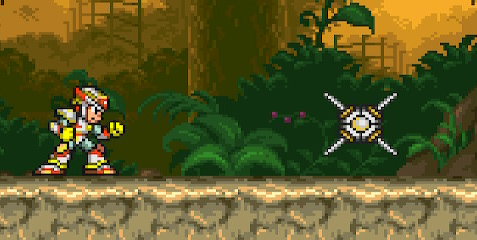
\includegraphics[height=3cm]{figures/X3/weapons/P_bomb.png}
		\caption{Normal fire}	
	\end{subfigure}
	\begin{subfigure}{.49\linewidth}
		\centering
		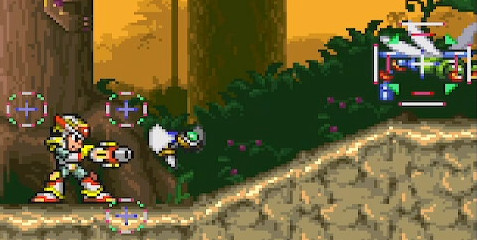
\includegraphics[height=3cm]{figures/X3/weapons/P_bomb_C.jpg}
		\caption{Charged version}	
	\end{subfigure}
	\caption{Parasitic Bomb sub-weapon}
\end{figure}


\subsection{
\includegraphics[width=12px, height=10px]{figures/X3/weapons/T_thunder.jpg} Triad Thunder}\label{Triad_Thunder}

The Triad Thunder is the weapon X obtains by defeating Volt Catfish~\ref{boss:Volt_catfish}. This sub-weapon generates three orbs around X in a triangular pattern which conducts electricity, forming a sort of shield. After few seconds the three orbs will fire stored electricity in their respective direction (up, diagonal-down left and diagonal-down right) and will then fall off-screen. It is possible, if the player has the right timing, to swap the orbs' position to form an upside-down triangle. With the correct timing it is also possible re-change the position to its original state, but it is important to note that for each change weapon ammunition is used. When charged X will punch the ground to release a shockwave which will deal massive damage to all enemies touching it. Moreover after the initial shockwave two electric sparks will part from X moving in opposite directions and following the ground.

\begin{figure}[htp]
	\centering
	\begin{subfigure}{3.9cm}
		\centering
		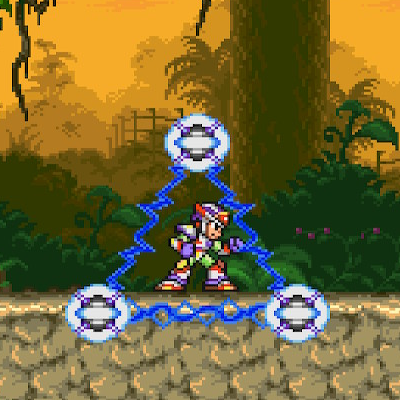
\includegraphics[height=3.5cm]{figures/X3/weapons/T_thunder.png}
		\caption{Normal fire}	
	\end{subfigure}
	\begin{subfigure}{3.9cm}
		\centering
		
\includegraphics[height=3.5cm]{figures/X3/weapons/T_thunder_3.png}
		\caption{Releasing electricity}	
	\end{subfigure}
	\begin{subfigure}{3.9cm}
		\centering
		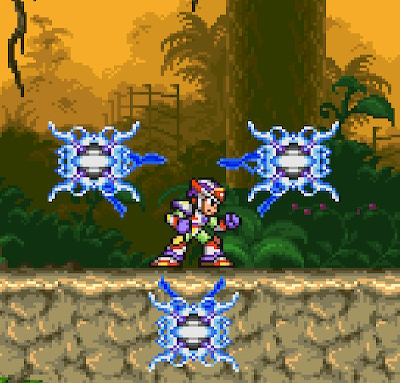
\includegraphics[height=3.5cm]{figures/X3/weapons/T_thunder_2.png}
		\caption{Upside-down formation}	
	\end{subfigure}
	\begin{subfigure}{\linewidth}
		\centering
		
\includegraphics[height=3.5cm]{figures/X3/weapons/T_thunder_C.png}
		\caption{Charged version}	
	\end{subfigure}
	\caption{Triad Thunder sub-weapon}
\end{figure}

\subsection{
\includegraphics[width=12px, height=10px]{figures/X3/weapons/S_blade.jpg} Spinning Blade}\label{Spinning_Blade}
When equipping this sub-weapon, the X buster will fire two spinning blade which travel forward for short amount of time, before curving backwards, one with an upward direction and the second downward. Due the particular trajectory of this weapon, using this weapon may result difficult at first, as its main use is to hit enemies behind X. However this weapon can also be used at close range in a shotgun-like way to make both blade hit a single enemy to deal massive damages. 
Upon charging, this weapon will release blade in a yo-yo style which will remain at a fixed distance from X as he moves. Upon pressing the UP or DOWN the blade will rotate in the  corresponding direction before returning to its original position. If while spinning the blade makes contact with an enemy it cannot destroy, the blade will bounce off, separating from the X-buster in the process.
This weapon is obtained after defeating Crush Crawfish (\ref{boss:Crus_crawfish}).

\begin{figure}[htp]
	\centering
	\begin{subfigure}{\linewidth}
		\centering
		
\includegraphics[height=3cm]{figures/X3/weapons/S_blade.png}
		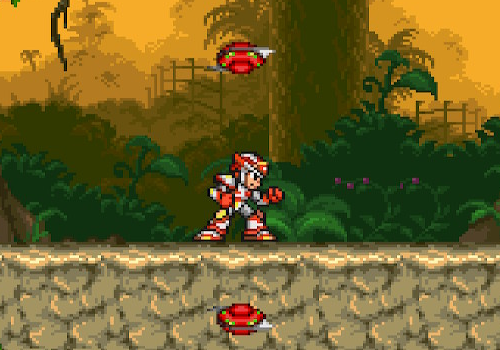
\includegraphics[height=3cm]{figures/X3/weapons/S_blade_1.png}
		\caption{Normal fire }	
	\end{subfigure}
	\begin{subfigure}{\linewidth}
		\centering
		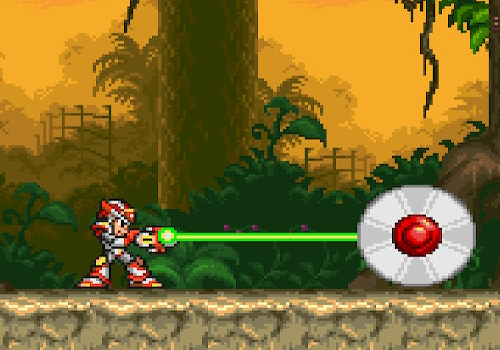
\includegraphics[height=3cm]{figures/X3/weapons/S_blade_C.png}
		
\includegraphics[height=3cm]{figures/X3/weapons/S_blade_C1.png}
		\caption{Charged version}	
	\end{subfigure}
	\caption{Spinning Blade sub-weapon}
\end{figure}

\subsection{
\includegraphics[width=12px, height=10px]{figures/X3/weapons/R_splasher.jpg} Ray Splasher}\label{Ray_Splasher}
The Ray Splasher is the weapon X obtains after defeating Neon Tiger (\ref{boss:Neon_tiger}). When using this weapon X will fire a volley of energy bullet in a spread formation. Upon charging this weapon X will release a glass container in the sky, which will shoot twenty-two Ray Splasher bullets in random direction.
\begin{figure}[htp]
	\centering
	\begin{subfigure}{.3\linewidth}
		\centering
		
\includegraphics[height=3cm]{figures/X3/weapons/R_splasher.png}
		\caption{Normal fire}	
	\end{subfigure}
	\begin{subfigure}{.3\linewidth}
		\centering
		
\includegraphics[height=3cm]{figures/X3/weapons/R_splasher_C.png}
		\caption{Charged version}	
	\end{subfigure}
	\caption{Ray Splasher sub-weapon}
\end{figure}
\subsection{
\includegraphics[width=12px, height=10px]{figures/X3/weapons/G_well.jpg} Gravity Well}\label{Gravity_Well}
When equipped with this sub-weapon, X will shoot a floating device which travels for a short distance before halting and activating a small high-gravity around it. Weak enemies which happen to be inside this area are instantly destroyed, while other enemies will remain untouched. After a few seconds the device will stop working and will return to X, which cannot fire another one until the first has returned. When charged, X will release a small black hole upwards, which will cause the gravity to shift up, carrying all weak enemies on screen alongside it. This weapon is acquired by X after defeating Gravity Beetle (\ref{boss:Gravity_beetle})
\begin{figure}[htp]
	\centering
	\begin{subfigure}{.25\linewidth}
		\centering
		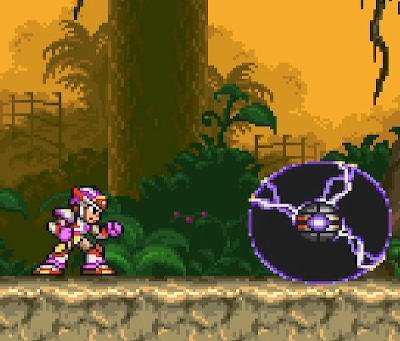
\includegraphics[height=3cm]{figures/X3/weapons/G_well.png}
		\caption{Normal fire}	
	\end{subfigure}
	\begin{subfigure}{.6\linewidth}
		\centering
		
\includegraphics[height=3cm]{figures/X3/weapons/G_well_C.png}
		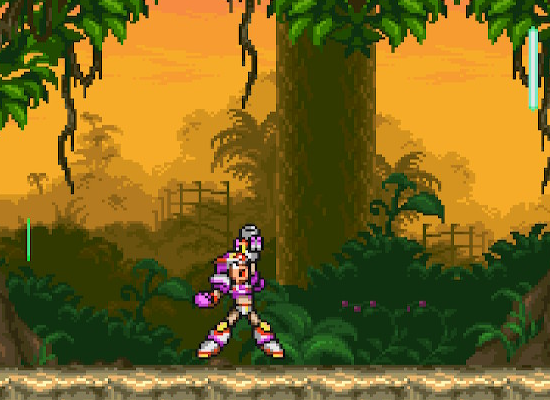
\includegraphics[height=3cm]{figures/X3/weapons/G_well_C_1.png}
		\caption{Charged version}	
	\end{subfigure}
	\caption{Gravity Well sub-weapon}
\end{figure}

\subsection{
\includegraphics[width=12px, height=10px]{figures/X3/weapons/F_shield.jpg} Frost Shield}\label{Frost_Shield}
Upon defeating Blizzard Buffalo (\ref{boss:Blizzard_buffalo}), X will gain access to the Frost Shield. When fired, this weapon will create a small icicle missile which moves forward after an initial delay. Upon making contact with a wall or an enemy the projectile will bounce off, creating a three-spiked trap on the ground which remain in position for few seconds before disappearing. X can fire up to two missiles at the time, but has to wait for the spikes to disappear before firing a third one. Upon charging X will create a spiked block of ice at the end of his X-buster which will deal damage to enemies which make contact with it and also acting as an effective shield, blocking incoming projectiles. After about nine seconds the shield will shatter and what remain will slide across the ground, but if X performs an air-dash the shield will immediately destroy.

When used underwater, the effects of this weapon change slightly: for the normal fire the missiles and spikes will have their size doubled, while the charged version replace the spiked shield with an ice boulder which float towards the surface and where X can stand on.

Finally, just like the Acid Burst (\ref{Acid_Burst}), this weapon too has the perks to guarantee health drop when destroying certain enemies (the same for which Acid Burst drops Ammo pickup), making it very effective for sub-tank filling.

\begin{figure}[htp]
	\centering
	\begin{subfigure}{3.9cm}
		\centering
		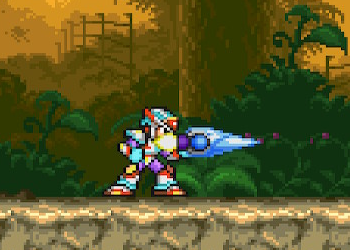
\includegraphics[height=2.7cm]{figures/X3/weapons/F_shield.png}
		\caption{Icicle Missile}	
	\end{subfigure}
	\begin{subfigure}{3.9cm}
		\centering
		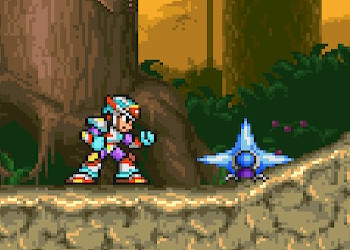
\includegraphics[height=2.7cm]{figures/X3/weapons/F_shield_1.jpg}
		\caption{Ice spike}	
	\end{subfigure}
	\begin{subfigure}{3.9cm}
		\centering
		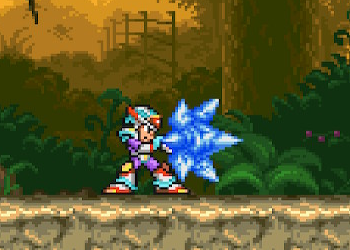
\includegraphics[height=2.7cm]{figures/X3/weapons/F_shield_C.png}
		\caption{Charged version}	
	\end{subfigure}
	\begin{subfigure}{3.9cm}
		\centering
		
\includegraphics[height=2.7cm]{figures/X3/weapons/F_shield_C_1.png}
		\caption{Shield remains sliding}	
	\end{subfigure}
	\begin{subfigure}{3.9cm}
		\centering
		
\includegraphics[height=2.7cm]{figures/X3/weapons/F_shield_C_2.png}
		\caption{Charged underwater }	
	\end{subfigure}
	\begin{subfigure}{3.9cm}
		\centering
		
\includegraphics[height=2.7cm]{figures/X3/weapons/F_shield_C_3.png}
		\caption{Using as a platform}	
	\end{subfigure}
	\caption{Frost Shield sub-weapon}
\end{figure}
%TODO picture of undwewater spikes

\subsection{
\includegraphics[width=12px, height=10px]{figures/X3/weapons/T_fang.jpg} Tornado Fang}\label{Tornado_Fang}
After defeating Tunnel Rhino (\ref{boss_Tunnel_rhino}),X will adapt the Tornado Fang into his arsenal. When used this weapon will fire a drill-shaped missile which briefly delays (just like the Frost Shield) before starting to move. Upon pressing the fire button again while the drill is stationary two more missiles can be spawned, for a total of three. Upon making contact with an enemy the missile will try to perforate the enemy, dealing constant damage in the process until its charge is depleted. If it successfully destroys an enemy it will keep moving forward until its charge is depleted. When charged this sub-weapon changes the X-buster into a drill until the fire button is pressed. While in this state X will deal damage to all enemies which make contact with it and, furthermore, the drill will also stick to the wall when X is wall jumping, allowing him to stay in place without sliding down.

\begin{figure}[htp]
	\centering
	\begin{subfigure}{\linewidth}
		\centering
		
\includegraphics[height=3cm]{figures/X3/weapons/T_fang.png}
		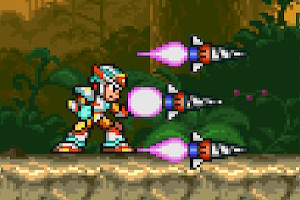
\includegraphics[height=3cm]{figures/X3/weapons/T_fang_1.png}
		\caption{Normal fire }	
	\end{subfigure}
	\begin{subfigure}{\linewidth}
		\centering
		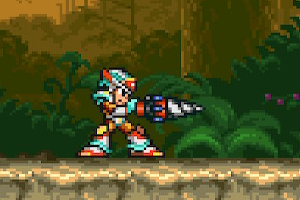
\includegraphics[height=3cm]{figures/X3/weapons/T_fang_C.png}
		
\includegraphics[height=3cm]{figures/X3/weapons/T_fang_C_1.png}
		\caption{Charged version + sticking to a wall}	
	\end{subfigure}
	\caption{Tornado Fang sub-weapon}
\end{figure}

\section{Third Armor + Beam-saber}\label{X3:Armor}

Following the trend of its predecessors, Mega Man X3 too offers to players a way to increase X's power through the usage of Armor Parts. This time, however, four more capsules can be found, bringing the total of hidden pieces up to eight, on per stage. Such additional capsules, painted in pink to distinguish them to regular ones, however do not contain actual armor parts but rather augment chip for a specific armor piece, which must be acquired first in order to obtain the power-up. The trade-off for such augment is, however, that the armor can only stand one of them and that they cannot be replaced, making the chosen upgrade permanent for the entire game. However, continuing the tradition of previous games, a final hidden capsule can be obtained as a prize for obtaining all collectible in the game, safe for said additional capsule. Such last capsule will give the player a special armor upgrade, which combines all the four optional chips into a single one, while also changing the armor color to gold. Finally, although not directly a part of the armor, there is another hidden upgrade X can obtain regardless of the armor status: the Beam-Saber

The Third armor (also known as Max Armor~\cite{wiki:third_armor}) is composed by the following parts:
\begin{itemize}
	\item Foot parts: Found in 	the Frozen Town Stage, near the end of the large area before the boss' room. This upgrade allows X to regain the air-dash ability in the same way as it was for the second armor. This time however the air dash can also be performed upwards, although with a short delay between the first and second jump. Just like the previous game, X cannot air-dash out of a dash-jump. It is possible, however, perform two upward dash, as it is not required for X to touch the ground before performing a second one.
	
	\begin{figure}[htp]
		\centering
		
\includegraphics[width=.45\linewidth]{figures/X3/Blizzard_buffalo/Armor_1.png}
		
\includegraphics[width=.45\linewidth]{figures/X3/Blizzard_buffalo/Armor_2.png}
		\caption{Armor Capsule location}
	\end{figure}
	
	\item Body Parts: Just like its predecessor, this part double X's defense by cutting in half all incoming damages. In addition, when X receives damage a blue force field appears around X for a short amount of time, reducing incoming damage for an additional 25\%, for a total damage reduction of 62.5\%. This upgrade is found in Volt Catfish's stage, on the vertical spiked pit after the fourth lift. It requires either a charged Gravity Well to lift the platform or the Foot Part with the upgrade chip (although it is not mandatory as it is possible to reach the upper ledge by combining two well timed upward dash).
	\begin{figure}[htp]
		\centering
		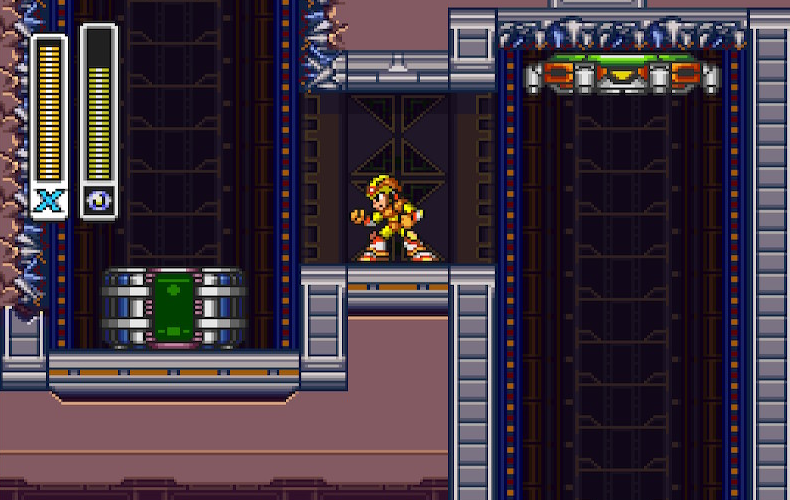
\includegraphics[width=.45\linewidth]{figures/X3/Volt_catfish/Armor_1.png}
		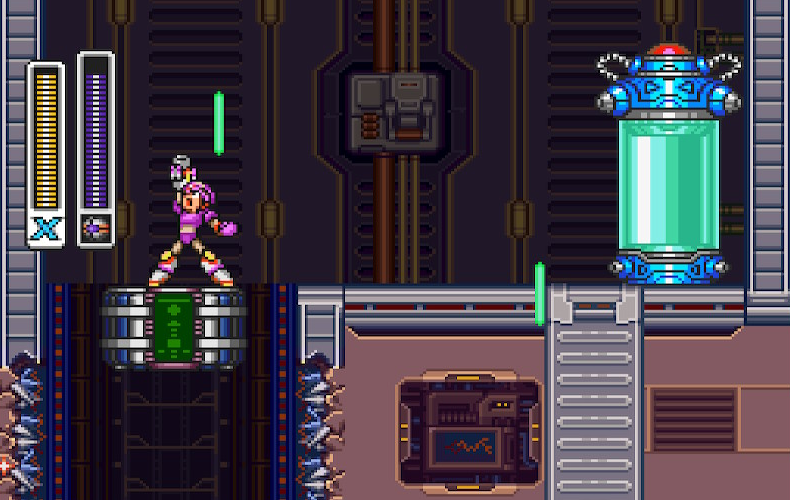
\includegraphics[width=.45\linewidth]{figures/X3/Volt_catfish/Armor_2.png}
		\caption{Armor Capsule location}
	\end{figure}
	
	\begin{figure}[htp]
		\centering
		
\includegraphics[height=3cm]{figures/X3/weapons/Armor_shield.png}
		\caption{Shield activated}
	\end{figure}
	
	\item Arm Parts: Increase X's maximum charge level up to four, while also allowing to charge sub-weapons. Similarly to he Second Armor, releasing a fully charged shot will cause X to shoot a single shot, while keeping a second one in store for later. It is also possible to release the second shot immediately after the second, just like in X2, but in this case the two shots instead of moving separately will combine in a single Cross Charged Shot. Although powerful, this attack also comes with some drawbacks, mainly the delay the two shots need to combine and start moving, which can cause to miss some potential opening in the enemies. 
	Beside the increase in attack power, the Arm Parts also X's to move faster on ladders, as well as cutting the ammo cost for sub-weapon in half, but only when the armor is fully completed. This part can be found in the Safari Park, behind a wall breakable by the Tornado Fang and a pit which requires a double dash to pass on.
	
	\begin{figure}[htp]
		\centering
		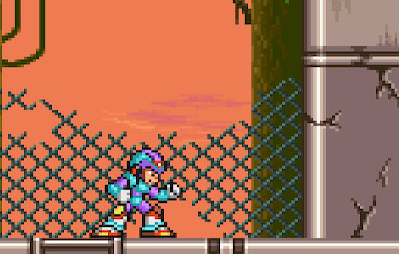
\includegraphics[width=.3\linewidth]{figures/X3/Neon_tiger/Armor_1.png}
		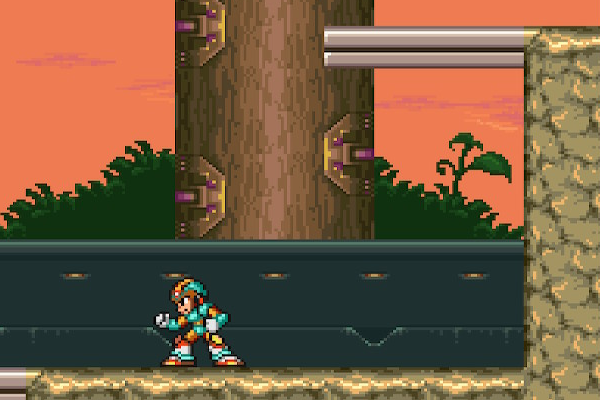
\includegraphics[width=.3\linewidth]{figures/X3/Neon_tiger/Armor_2.png}
		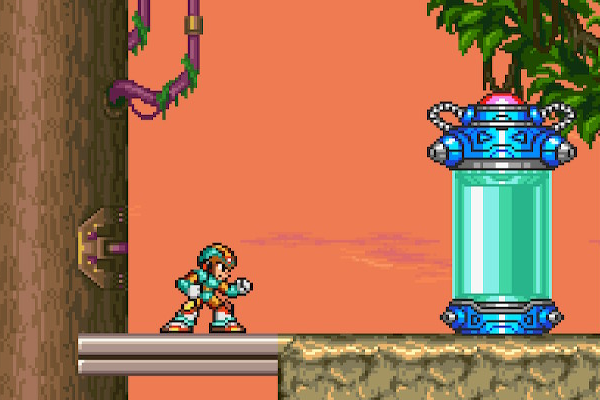
\includegraphics[width=.3\linewidth]{figures/X3/Neon_tiger/Armor_3.png}
		\caption{Armor Capsule location}
	\end{figure}
	
	\begin{figure}[htp]
		\centering
		
\includegraphics[height=3cm]{figures/X3/weapons/Combo_shot.png}
		\caption{Cross charged shot}
	\end{figure}
	
	\item Head Parts: Found in Tunnel Rhino's stage, in a path opened by a boulder fall after using the charged Triad Thunder. This parts will add a radar to X's equipment which will map the current stage's layout and point out yet-to-discover collectibles, such as other armor capsule, life-up and sub-tanks. The map is displayed only once as soon as X enters a stage, but it requires an input for the player to close, so it can remain on screen for as much as the player wants. Additionally, on the stage selection screen additional information for each stage will be displayed, showing collectibles for each stage and highlighting missed ones.
	
	\begin{figure}[htp]
		\centering
		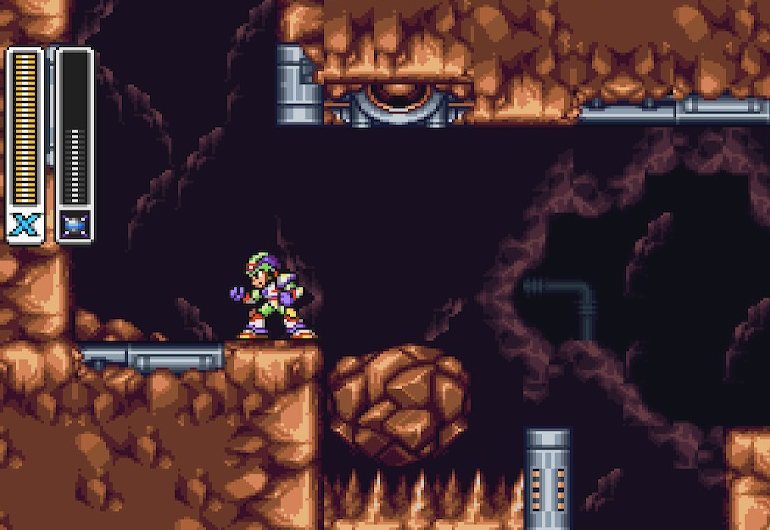
\includegraphics[width=.45\linewidth]{figures/X3/Tunnel_rhino/Armor_1.png}
		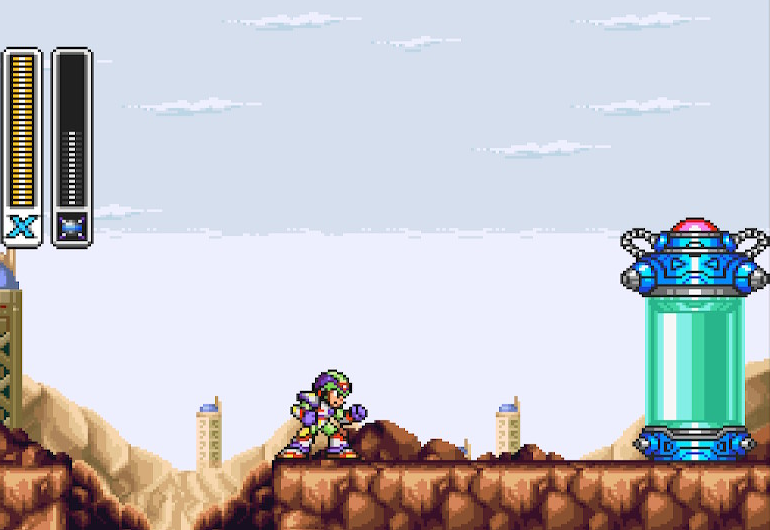
\includegraphics[width=.45\linewidth]{figures/X3/Tunnel_rhino/Armor_2.png}
		\caption{Armor Capsule location}
	\end{figure}
	
	\begin{figure}[htp]
		\centering
		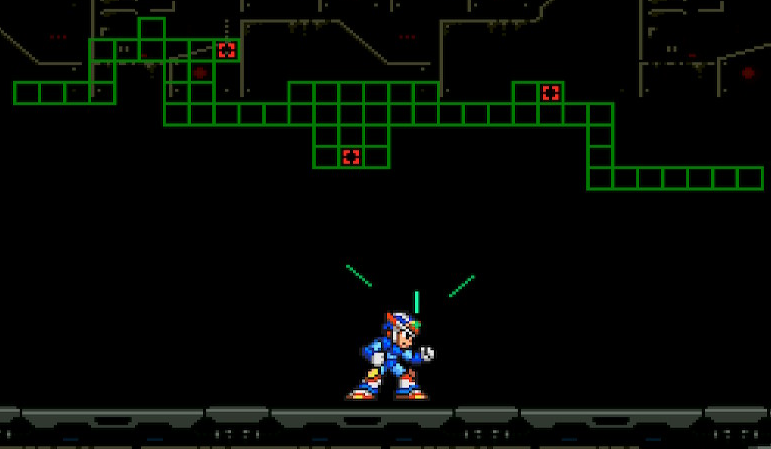
\includegraphics[height=3cm]{figures/X3/Blast_hornet/map.png}
		\caption{Map layout displayed}
	\end{figure}
	
\end{itemize}

As said previously, for each part an upgrade chip can be installed. Hence there are four total chip upgrades, plus a hidden fifth one. the chips are the following:
\begin{itemize}
	\item Foot Chip: Found in Toxic Seahorse's stage, on the surface of the big underwater room on the right. It requires either the charged Frost Shield to reach the surface and jump from there or the Frog Ride Armor, to destroy the fans which prevent X to wall jump on the rightmost wall. The Chip allows X to perform a second air dash in any direction, or an air-dash out of a dash-jump.
	\begin{figure}[htp]
		\centering
		\includegraphics[height=3cm]{figures/X3/Toxic_seahorse/Armor_1.png}
		\includegraphics[height=3cm]{figures/X3/Toxic_seahorse/Armor_2.png}
		\caption{Foot Chip location}
	\end{figure}
	\item Body Chip: Increase the power of the force field emitted by the part after receiving a hit. The shield now becomes orange, and cut damages by another 50\%, for a total of 75\% damage reduced. This chip can be found in the Shipyard stage, in a passage down a pit closed by a wall breakable only by using a Ride Armor.
	\begin{figure}[htp]
		\centering
		\includegraphics[height=3cm]{figures/X3/Crush_crawfish/Armor_1.png}
		\includegraphics[height=3cm]{figures/X3/Crush_crawfish/Armor_2.png}
		\caption{Body Chip location}
	\end{figure}
%TODO orange shield
	\item Arm Chip: Allows the usage of the Hyper Charge, which grants unlimited charged shots as long as there is weapon energy available. The chip is found in Gravity Beetle's stage, at the end of a spiked path blocked by crates breakable only by using a Ride Armor.
	\begin{figure}[htp]
		\centering
		\includegraphics[height=3cm]{figures/X3/Gravity_beetle/Armor_1.png}
		\includegraphics[height=3cm]{figures/X3/Gravity_beetle/Armor_2.png}
		\caption{Arm Chip location}
	\end{figure}
	\item Head Chip: Enable health regeneration when X stand still. When X remain standing for a while his health will begin to regenerate and the regeneration will continue for as long as he doesn't move. If X is at full health, the regeneration effect will replenish his sub-tanks instead. This chip is found in the Weapons Factory Stage, at top-right side of the area past the elevator, accessible by using the Falcon Module for the Ride Armor.
	\begin{figure}[htp]
		\centering
		\includegraphics[height=3cm]{figures/X3/Blast_hornet/Armor_1.png}
		\includegraphics[height=3cm]{figures/X3/Blast_hornet/Armor_2.png}
		\caption{Head Chip location}
	\end{figure}
	\item Hyper Chip: Obtainable only if X has obtained all the collectibles and has not installed any other chip. Once obtained, X's armor turns gold and X gets access to all the previous upgrades, with the addition of having an increased health regeneration and a less usage of energy when in Hyper Charge. The capsule for the chip is hidden in Doppler Stage A, in a secret room inside a pit but only if the player reaches it at full health. This upgrade is NOT saved by the password system. 
	\begin{figure}[htp] %TODO better hyper chip screenshot
		\centering
		\includegraphics[height=3cm]{figures/X3/Doppler_stages/Hyper_chip.png}
		\caption{Hyper Chip location}
	\end{figure}
\end{itemize}

The last upgrade X can obtain is the beam saber. This upgrade can be obtained independently from the armor's status, as the actions required to obtain it can be done even by regular X. However obtaining this upgrade while also having the Arm Parts will increase its power.

The path which leads to obtain the Beam Saber is rather straightforward, and obtainable with the following steps:
\begin{itemize}
	\item Find and defeat Vile mk.II using one of his weakness, killing him in the process.
	\item By killing Vile, the Doppler Stage B will change accordingly. In the new path X will find the sub-boss  \hyperlink{miniboss:Mosquittus}{Mosquittus}. This is the only sub-boss Zero can fight and, upon defeating it, the boss will self-destruct after trapping Zero. This will cause Zero to be seriously damaged (preventing him to be called again) but in exchange he will give X his Beam Saber.
\end{itemize} 
The Beam Saber gives X another level in his charge shot, which turns green. Upon releasing the fire button, X will swing the beam saber dealing massive damage to every enemy he hits with it. If X is equipped with the Arm Part, the saber will also produce a shockwave which travels forward, and upon making contact with an enemy will not only deal heavy damages to the target, but also produce three more slashes which will deal even more damage over time. In particular, hitting any enemy with the saber itself will deal 30 damage per frame to all enemies whereas a fully charged saber will deal a total of 98 damages. When fighting bosses, the regular saber will deal 16 damages (half health bar), while de shockwave will deal 8 damages, followed by three slashes which deals 4 damages each, dealing in total 20 damages.

\begin{figure}[htp] 
	\centering
	\includegraphics[height=3cm]{figures/X3/weapons/Z_saber_1.png}
	\includegraphics[height=3cm]{figures/X3/weapons/Z_saber_2.png}
	\caption{Z-Saber swing and shockwave}
\end{figure}

\section{Zero Change}\label{X3:Zero}
A new feature added to the game is the Zero change~\ref{wiki:Zero_change}, which gives the player the ability to play temporary as Zero. From the pause menu, by pressing the L button a secondary screen will appear which can be used to call for Zero. If the player decides to deploy him, Zero will replace X and become playable. 
\begin{figure}[htp] 
	\centering
	\includegraphics[width=.5\linewidth]{figures/X3/weapons/Zero_screen.png}
	\caption{Zero change menu}
\end{figure}
There are, however, some restriction on when Zero can be used:
\begin{itemize}
	\item Zero can only deployed once per stage. If X switches back in, for any reasons, it is impossible to switch again to Zero until the player gets a game over or exits the stage.
	\item Zero cannot engage fight with any bosses or sub-bosses, except for Mosquittus. Upon reaching a boss door, the game will automatically swap back to X.
	\item If Zero dies for any reason, he will become unusable for the rest of the game.
\end{itemize}

Generally speaking, Zero plays similarly to X, but sacrificing defenses for more firepower. Zero in fact, despite possessing more HP than X even after all upgrades are obtained, does not possess any armor upgrade, meaning that enemies will always do full damage to him and depleting his HP quicker than X. In terms of firepower, the Z-buster Zero comes with behave very similarly to the Arm Parts of the third armor, Z-saber included. Zero can charge his shots up to five level, the latter being the saber swing, but the lack of access to sub-weapons greatly limit his fighting options. Also since Zero is a little taller than X, his shots will also be higher. Finally as Zero the player is not able to obtain any collectible, nor can use ride armors.


\begin{figure}[htp]
	\centering
	\begin{subfigure}{\linewidth}
		\centering
		\includegraphics[width=.4\linewidth]{figures/X3/weapons/zero_shot_1.png}
		\includegraphics[width=.4\linewidth]{figures/X3/weapons/zero_shot_2.png}
	\end{subfigure}
	\begin{subfigure}{\linewidth}
		\centering
		\includegraphics[width=.4\linewidth]{figures/X3/weapons/zero_shot_3.png}
		\includegraphics[width=.4\linewidth]{figures/X3/weapons/zero_shot_4.png}
		\caption{Charged version + sticking to a wall}	
	\end{subfigure}
\begin{subfigure}{\linewidth}
	\centering
	\includegraphics[width=.5\linewidth]{figures/X3/weapons/zero_shot_5.png}
\end{subfigure}
	\caption{Zero's charged shots levels.}
\end{figure}

\section{Opening Stage: Hunter Base}\label{X3:intro_stage}
Few hours after X and Zero are dispatched to Doppler Town, dr.~Doppler's army attack directly the Maverick Hunters HQ, forcing the two to quickly retreat to defend their base, which became the first stage of the game. The stage itself is rather straightforward, as its focus on reintroducing the core mechanics of the series. At about one third of the stage X will meet with Mac, a former Maverick Hunter now member of Doppler's army, which betrays captures X. At this point the game introduces for the first time the Zero Change, forcing the player to take control of Zero for the remaining of the stage. Near the stage's end the player will find Mac as a sub-boss, but it can be easily destroyed thanks to Zero's firepower. Once destroyed Mac and freed X, the player will regain control of the latter, to reach the end of the stage and face the boss, Mao the Giant.

This stage houses  the following enemies~\cite{wiki:X3_opening}:
\begin{itemize}
	\item \hyperlink{enem:Hangerter}{Hangerter}
	\item \hyperlink{enem:Notor_Banger}{Notor Banger}
	\item \hyperlink{enem:Head_Gunner_customer}{Head Gunner customer}
	\item \hyperlink{enem:Caterkiller}{Caterkiller}
	\item \hyperlink{enem:Earth_Commander}{Earth Commander}
\end{itemize}

\subsection{Maoh the Giant}\label{boss:Mao_the_giant}
Similar to the opening stage of X2, X3 also ends first stage with a fight against a giant mechaniloid. Named "Maoh the Giant", this particular mechaniloid belonging to Doppler's army is stated to be the size of an entire building~\cite{wayback:X3_resources} and was dispatched to attack the Maverick Hunters HQ, before X and Zero quickly returned to destroy him. 

Although colossal, the fight against Maoh the Giant is relatively easy, considering its only way to attack the player it has is to ram the wrecking ball on the arms towards the player, but they only cause 1 point of damage,a although they leave a crater on the impact point, breaking the arena. Luckily for the player these big spike balls are also Maoh weak point, and together with the fact that its attack are relatively slow, it is very easy to bait an attack, dodge it and hit the spike ball with a charged shot.

\section{Weapons Factory}
The first stage the game points to is the weapon factory stage, where Blast Hornet resides. Although not easy to beat, it is often suggested to face this stage first or second, as beating it lowers significantly the difficult due and the collectibles found as well as the  stage interactions which happens upon beating the stage.

The stage itself can be divided into three segments: two inside the factory (first and third) an one outside (the second). The stage's first section consists in a ride with an elevator while avoiding enemies shooting from above, followed by a descend onto conveyor belts which tries to push X either into pits or towards spikes. At the end of this first part there is a mini-boss fight against \hyperlink{miniboss:Shurikein}{Shurikein}, a 3D wireframe shuriken. Shurikein's main attacks consists in rolling across the stage back and forth or up the walls, or bouncing while spinning (but only at low health). The best way to deal with this miniboss is to deal as much damage as possible in the shortest amount of time, to avoid prolonging the fight. To do so, the Acid Burst is the best option as it can dispose of the boss in six hits. 

Passed the miniboss, the second segment of the stage begins. This part takes place on the outside, on the roof of some warehouses with enemies coming from above. In between the roofs there are some platforms with crates on them which, if destroyed, will blow up the platform too and open a passage to the warehouse's basement. Here by using  the Tornado Fang sub-weapon it is possible to destroy the cracked walls and proceed forward without having to face enemies on the roof. Passed the last warehouse there is a long stretch of road where, if the player has not yet defeated Gravity Beetle, an airship will appear to load the cargo. The player must destroy the boxes that the \hyperlink{enem:Carry_Arm}{Carry Arm} enemies delivers to avoid the spawn of enemies and also to proceed in the stage. After enough boxes have been destroyed the cargo will flee, allowing X to proceed in the stage.

The last portion of the stage is again an inside section, with more conveyor belt and spikes, but with the addiction of large pile of crates blocking the path and that, once destroyed, open pits with crates falling regularly into them, requiring the player to jump at the correct time to avoid getting hit. Once even this section has been passed, the player will reach the boss door leading to Blast Hornet.

Following enemies populate the stage~\cite{wiki:Weapon_factory}, while figure~\ref{fig:Weapon_factory_map} shows the stage's layout:
\begin{itemize}
\item \hyperlink{miniboss:Genjibo}{Genjibo} and \hyperlink{miniboss:Shurikein}{Shurikein}
\item \hyperlink{enem:Carry_Arm}{Carry Arm} (before completing Gravity Beetle's stage)
\item \hyperlink{enem:Hangerter}{Hangerter} (holding Ride Armor)
\item \hyperlink{enem:Head_Gunner_customer}{Head Gunner customer} (before completing the stage)
\item \hyperlink{enem:Head_Gunner_masspro}{Head Gunner masspro} (after completing the stage)
\item \hyperlink{enem:Helit}{Helit}
\item \hyperlink{enem:Meta_Capsule}{Meta Capsule} (before completing Gravity Beetle's stage)
\item \hyperlink{enem:Notor_Banger}{Notor Banger}
\end{itemize}

After defeating this stage two main changes will trigger: All metal crates in Gravity Beetle stage will disappear, opening the path to the Heart Tank, and all the Head Gunner customer enemies in the remaining stages (except for final ones) will be downgraded to their masspro version, easier to deal with.

\subsection{Head Chip Capsule}
The Head Chip power-up is hidden in the first conveyor belt room, in the top-right corner. It is, however, protected by a wall covered in spikes which can only be bypassed by using the Leg parts or the dash of the Hawk Ride Armor, which can be summoned earlier in the stage.

\subsection{Ride Armor Chimera}
In the outside section by dropping down the roof after destroying the boxes on the platform connecting the first roof with the second, it is possible to note that all walls of the warehouses are cracked. It such walls are hit with the Tornado Fang they will break and open a new passage. In particular, in the second warehouse there is a box that, once destroyed, will open an underground path that leads to the ride armor, imprisoned by an \hyperlink{enem:Hangerter}Hangerter. Destroying such enemy will free the armor, which will become usable immediately

\subsection{Heart Tank}
The Heart Tank is hidden at the end of the outside area, in the top right corner of the map. To reach it it is necessary use the Ride Armor to jump out of it while in midair, to let X gain enough height to reach the upper wall and beginning to wall-jump.

\subsection{Blast Hornet}\label{boss:Blast_hornet}
Also known as the ``\textit{Flying Shadow Ninja''}, Blast Hornet was the second in command of the Maverick Hunter's 0th division (Shinobi Unit). When Dr.~Doppler invited Zero to come to Doppler Town, he declined the invitation as he was busy training~\cite{wayback:X3_resources}, therefore Hornet was sent instead. Once known  for his calm composure and cool judgment~\cite{wiki:Blast_hornet}, Hornet fell victim of the Sigma Virus which spread throughout the city, causing him to change into a merciless soldier of Doppler's army. Hornet was then sent to guard Doppler's weapon factory, where he fought and was destroyed by the hand of X.

Blast Hornet will spend most of his boss fight by flying in the air around the stage. He possesses only three attacks, but all of them can become deadly due the high damage they deal. During the first phase, Hornet will cycle only between two attacks, his \emph{Sting Attack}~\cite{book:Compendium}, where Hornet dives toward X trying to hit him with his stinger, and the \emph{Mini Bee Summon}~\cite{book:Compendium}, which sees Hornet creating five mini bees which will scatter towards X. When a mini bee makes contact with X or a wall it will stick to it, only to explode shortly after. Finally, at about half health, Hornet will also begin using is \emph{Search Attack}~\cite{book:Compendium}. With this attack a pink crosshair will appear on the screen and home onto X, while Hornet will begin summoning mini bees around him. If the cursor locks onto X, all the bees around Hornet will home to X, causing heavy damages. Moreover, for the entire duration of the fight, Hornet will keep flying in a $\infty$ patter which will become larger as his health drop. Near the end Hornet will fly almost at ground level, making him easier to hit but also harder to avoid all his attacks.

There are two main strategies to deal with Blast Hornet, depending on whether the player has access to Hornet's weakness, the Gravity Well. If such weapon is not available, the best strategy possible is to avoid as much attacks as possible, and to deal damage only when Hornet exposes himself. The best way to do so is to destroy all the mini bees as he summons them whit a charged shot after a wall jump (when they are still all near, which will cause the single shot to destroy all of them and also hit Hornet), bait the Stinger attack, avoid it and hit Hornet again with another Charged Shot. The same strategy can also be applied in the second phase, although with more difficulties due the increased movement. A different approach can be adopted instead should the player have obtained the Gravity Well. This weapon can completely shut down all Hornet's attack, as using hit will stun and bring him to the ground, while also destroying all the bees on screen. Furthermore it is also possible to almost permanently stun Hornet for the whole fight, just by putting X close enough to the Gravity Well to reduce the time needed by the weapon to return to X and be available again.

According to data available~\cite{wayback:X3_resources}, Blast Hornet is 242 cm tall, weights 65 Kg, has a power of 3400 rp and a speed of 8600 rp. Upon defeating him X will gain access to the Parasitic Bomb~\ref{Parasitic_Bomb}.

\section{Frozen Town}
\section{Airborne Aircraft Carrier}
\section{Giant Dam}
\section{Power Control Center}
\section{Shipyard}
\section{Quarry}
\section{Safari Park}

\section{Doppler Stage 1}
\section{Doppler Stage 2}
\section{Doppler Stage 3}

\section{Miscellaneous}\label{X3:misc} %